\documentclass{article}

\usepackage{graphicx} % Required for the inclusion of images
\usepackage{natbib} % Required to change bibliography style to APA
\usepackage{amsmath} % Required for some math elements 
\usepackage[final]{pdfpages}
\usepackage[parfill]{parskip}
\usepackage{bm}

\usepackage[utf8]{inputenc}
\usepackage{mathpazo}
\usepackage[T1]{fontenc}
\usepackage{textcomp}
\usepackage{gensymb}
\usepackage{mathtools} 
\usepackage{algorithm}
\usepackage{algpseudocode}
\usepackage{fancyhdr}
\usepackage{booktabs}

\usepackage{amsmath,amsfonts,amssymb}

\setlength\parindent{0pt} % Removes all indentation from paragraphs

\renewcommand{\labelenumi}{\alph{enumi}.} % Make numbering in the enumerate environment by letter rather than number (e.g. section 6)

\long\def\/*#1*/{}

%----------------------------------------------------------------------------------------
%	DOCUMENT INFORMATION
%----------------------------------------------------------------------------------------

\title{Embedded Agent for Power-sensitive Arm Control} % Title

\author{\textsc{Nick Walker}} % Author name

\date{CS394R Fall 2016} % Date for the report

\begin{document}
	
\maketitle % Insert the title, author and date


%----------------------------------------------------------------------------------------
%	SECTION 1
%----------------------------------------------------------------------------------------

\section{Motivation}

Embedded agents, which face memory and compute constraints, have applications in many areas, including space and consumer electronics. There are significant challenges in adapting reinforcement learning approaches for the constraints of embedded devices. In a previous programming assignment, I solved a simple task on a memory-constrained two-joint arm system using a temporal difference learning approach. This was successful because it was possible to achieve reasonable performance with even a coarse representation of the state and action spaces. In many problems however, acceptable performance can only be attained with finer representations. In this assignment, I increase the difficulty of the task while maintaining memory constraints and survey how a learning approach might be applied.


%----------------------------------------------------------------------------------------
%	SECTION 2
%----------------------------------------------------------------------------------------

\section{Introduction}

\subsection{Learning Platform}

I based the platform on the Teensy 3.2, an ARM Cortex-M4 development board. The Teensy's particular M4 has 256kb of program memory, 64kb of SRAM and operates at 72MHz. It is 32-bit and has a floating point unit. Compared to popular 8-bit AVR microcontrollers, ARM chips are substantially more powerful, and not much more expensive. The Cortex line has seen substantial commercial use, so evaluating an embedded agent using the M4 provides useful insight what the constraints of real systems are.

In order to provide a challenging task for the agent, I built a six degree of freedom arm. The arm's joints are MTR955 servos, each capable of 170$\degree$ of rotation, though some joints have less range of motion to physical constraints.


\begin{figure}
	\centering
	%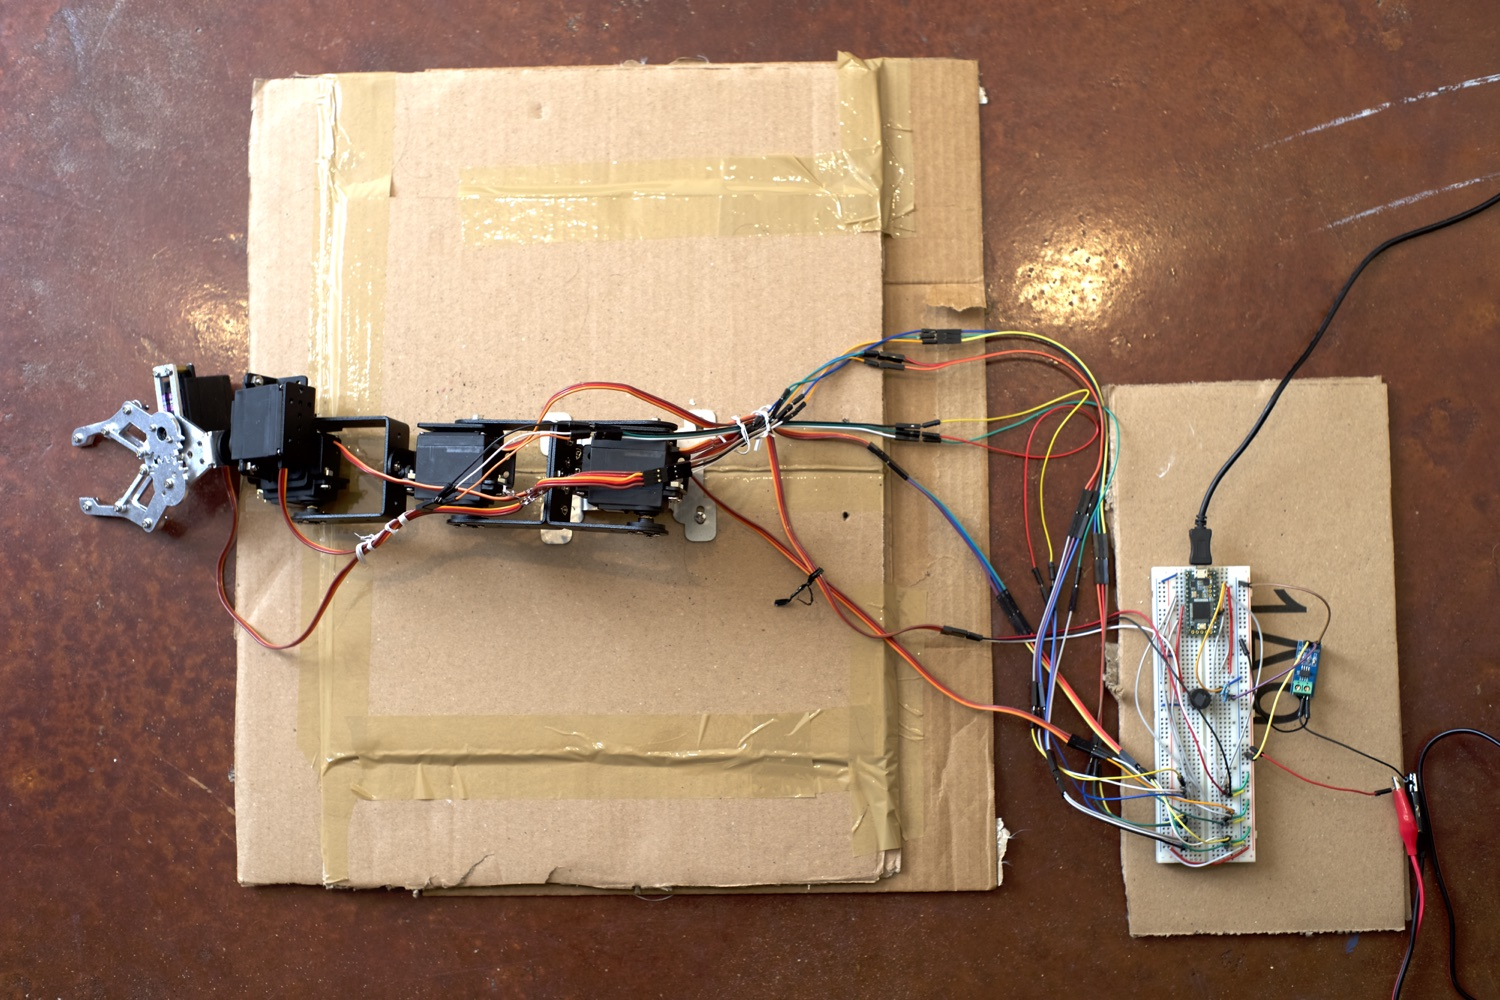
\includegraphics[width=10cm]{../photos/eagle_small.jpg}
	%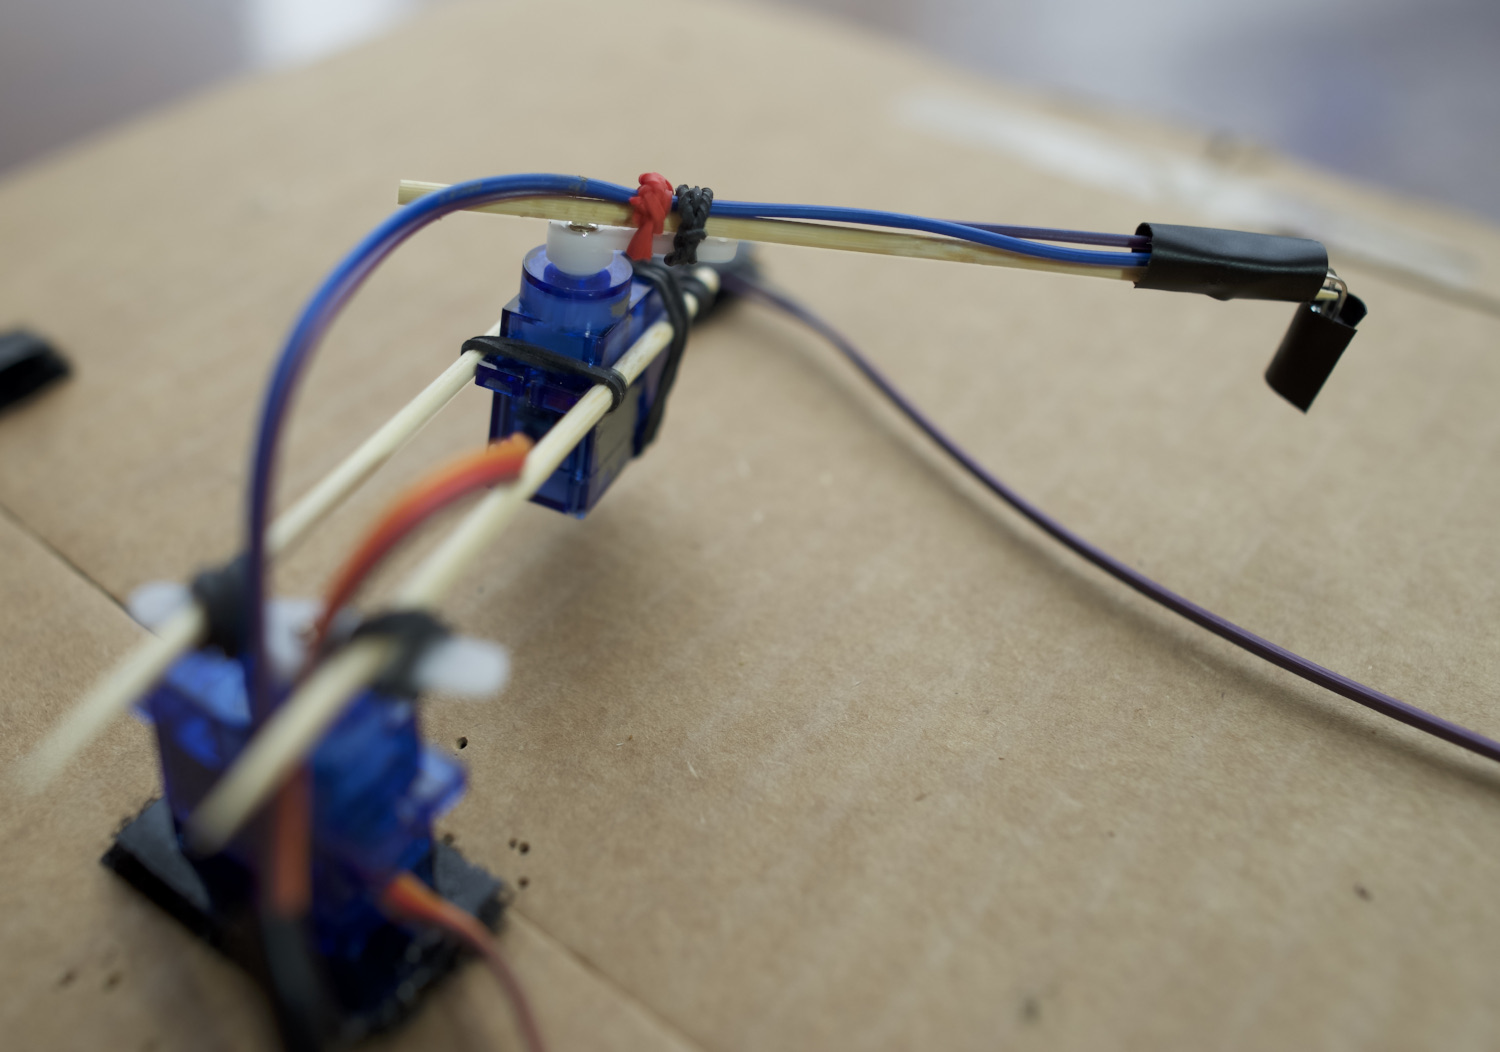
\includegraphics[width=10cm]{../photos/arm_detail_small.jpg}
	\caption{Top: The learning platform.}
	\label{fig:platform}
\end{figure}


\subsection{Problem}

Motors consume a substantial amount of power.

Additionally, power consumption is an interesting proxy for joint state. I did not use feedback servos, so it is not possible to know whether a joint has been able to execute its movement. The agent must assume that all actions get executed within some fixed window after they are issued. If the arm enters a bad configuration, e.g. hitting an immovable object, power consumption will spike as the servo controller applies more torque.

The agent must move all of its joints into a target pose, using as little energy as possible. A sample of the instantaneous current usage is taken during each action execution.

\[ r(s,a,s') =  \left\{
\begin{array}{ll}
	50 & \text{if all joint angles are match the target pose} \\
	-current & \text{otherwise} \\
\end{array} 
\right. \]


\subsection{Learning Approaches}

\subsection{Value Function?}

The problem suggests The servo control library used for this project allows motor targets to be set with single-degree precision, so a single joint can have integer positions in  $[0\degree, 155\degree]$.

\subsubsection{Policy Gradient}



The servo control library used for this project allows motor targets to be set with single-degree precision, so a single joint can have integer positions in  $[0\degree, 155\degree]$. For each configuration, the LED can be either on or off, so there are a total of 48050 states. At a given time step, the agent may choose to keep a joint fixed, move it left, or move it right and it can choose to activate or deactivate the LED. Assuming we restrict the agent to movements of unit magnitude, this means there are eighteen actions.

A state-action value table based on this representation, assuming 4 byte floats, would occupy more than 4 megabytes of memory. Due to the spread of the light of the LED, it may be feasible to reduce the fidelity of the joint state representation and still achieve good performance, and because the optimal policy will likely always elect to move a joint, we may be able to remove actions which do not move a joint with little adverse effect. Even then, the microcontroller could only theoretically fit 10\% of all state action pairs (less without careful optimization, as the stack needs to live in memory as well). A tabular approach is not feasible due to the system's memory constraints.

\subsubsection{Function Approximation}

Approximation allows tight control of the amount of memory being used to represent the value function. Because of the complex update step however, only at most half of the memory can be used for storing weights. Even then, the update step must be implemented carefully to control the stack size. Consider the episodic semi-gradient one-step Sarsa update:

\begin{equation}\label{eqn:update}
\bm{\theta}_{t+1} = 
\bm{\theta}_t + 
\alpha \Big[
	R_{t+1} + 
	\gamma \hat{q}(S_{t+1}, A_{t+1}\, \bm{\theta}_t) 
	- \hat{q}(S_t, A_t, \bm{\theta}_t)
\Big]
\nabla\hat{q}(S_t, A_t, \bm{\theta}_t)\tag{1}
\end{equation}

And in the linear case:

\begin{equation}\label{eqn:linear_update}
	\bm{\theta}_{t+1} = 
	\bm{\theta}_t + 
		\alpha \Big[
			R_{t+1} + \gamma\, \bm{\theta}_t^\top\bm{\phi}_{t+1} \space
			- \bm{\theta}_t^\top\bm{\bm{\phi}}_t
		\Big]\bm{\bm{\phi}}_t\tag{2}
\end{equation}

It is possible to implement the update using only $n$ additional space, where $n$ is the number of weights, but this is easy to do incorrectly. If the action selection step is placed after the memory allocation, the stack will consume $2n$ memory; maximizing the value function over possible next states requires an additional $n$ stack space.

	\begin{algorithm}
		\caption{Memory-conscious Episodic Semi-gradient One-step Sarsa}
		\label{alg:update}
		\begin{algorithmic}[1] % The number tells where the line numbering should start
			\Procedure{Update}{$S_t$, $A_t$, $S_{t+1}$, \bm{$\theta$}}
			\State $A_{t+1} \gets $ choose action from $S_{t+1}$ according to policy
			\State Allocate \bm{$x$} to be a vector the size of \bm{$\theta$}, and floats $r$ and $a$
			\State $r\gets r(S_t$, $A_t$, $S_{t+1}$)
			\State $\bm{x} \gets \bm{\phi}(S_{t+1}, A_{t+1})$ \Comment store $\bm{\phi}_{t+1}$
			\State $a \gets \bm{\theta}^\top \bm{x}$ \Comment calculate $v(S_{t+1},A_{t+1})$ so we can discard $\bm{\phi}_{t+1}$
			\State $\bm{x} \gets \bm{\phi}(S_{t}, A_{t})$ \Comment store $\bm{\phi}_t$
			\State $a \gets r + \gamma v - \bm{\theta}^\top \bm{x}$ \Comment $a$ is now the bracketed term in eq. $\ref{eqn:update}$
			\State $\bm{x} \gets (\alpha \space a)\bm{x}$ \Comment $\bm{x}$ is now the weight update
			\State \bm{$\theta} \gets \bm{\theta} + x$
			\
			\EndProcedure
		\end{algorithmic}
	\end{algorithm}
	
An approximation approach implemented on the microcontroller can use at most 1kb of RAM, or 250 features (less the incidental stack space required during the update step). It was not clear that this would be sufficient for good performance, but it was the only feasible approach. I implemented a semi-gradient one-step Sarsa agent using a linear function approximator.
	
I have not dwelt on time efficiency since, even with software floating point operations, 16MHz permits a fair amount of computation. For this project, I was satisfied as long as actions could be selected more quickly than the servos could execute them. Meeting this deadline, which was about 100ms, or 1.6 million cycles, was not an issue, even while the device was also streaming logging information over serial. If time performance requirements were tighter, special attention would need to be paid to the action selection process, which involves $|A|$ value function queries, each costing $n$ multiplications
	
	

%----------------------------------------------------------------------------------------
%	SECTION 3
%----------------------------------------------------------------------------------------

\section{Experimental Setup}


The agent learns for 50 episodes using $\alpha =$ 0.2, $\gamma =$ 0.99,  following an $\epsilon$-greedy policy with $\epsilon=$ 0.1. Then, the agent operates in an evaluation mode for 50 episodes with $\alpha=\epsilon=0.0$. During this period, episodes are limited to 200 steps in case the agent executes a policy that never reaches the goal. A small delay is used between action execution and sensing to allow the arm to settle. The photocell threshold is calibrated before every session to prevent spurious activations.

\subsection{Features}

I used a simple discretization of the state space. The range of each joint was divided into 8\space\space20\degree\space sections. The two sets of section features along with a binary feature for the LED state were then gridded, resulting in 128 mutually exclusive binary features. 

Because of the large number of actions, it was not feasible to maintain separate approximators per action, so I used three action features: two characterizing the direction of each joint's movement, taking values in $\{0, 1, -1\}$, and one binary feature describing whether or not the LED is activated by the action. Clearly, three features is insufficient to encode the differences in value for all actions across the state space, however there was not enough memory to grid these features with the state features. The total number of weights in the representation is still below the theoretical maximum number of weights for the microcontroller, so additional features could have been added with more time.


\subsection{Actions}

At each time step, the agent selects one entry from each column to form its action. If the LED is already on and the agent chooses an action that includes turning the LED on, the light remains activated for the next timestep. The behavior is symmetric in the LED off case.

\begin{center}
	\begin{tabular}{ l l l}
		Joint 1 & Joint 2 & LED\\ \midrule
		Move left & Move left & Turn on\\
		Move right & Move right & Turn off\\
		No movement & No movement & 
		
	\end{tabular}
\end{center}

To better support the state representation, I set the agent's movement increment to 20\degree. This ensures that the state resulting from any movement has a different feature vector than the previous state. This change does limit the granularity of the agent's movements, but without it, the agent must randomly escape the 20\degree\space sections by repeatedly making smaller movements, which makes learning take much longer. 

%----------------------------------------------------------------------------------------
%	SECTION 4
%----------------------------------------------------------------------------------------


\section{Results}


	\begin{figure}[h]
		\begin{center}
			%\includegraphics[width=\textwidth]{figure_0.pdf}
			\caption{The agent's performance. The first 50 episodes are learning time, the rest are evaluations. Due to the time expense of collecting data from the robot, I could only run ten trials. Still, within reasonable confidences, the agent's evaluation averages a reward of 44, demonstrating that it was able to quickly point the LED towards the photocell from arbitrary start positions.}
		\end{center}
	\end{figure}
	
\subsection{Discussion}

The agent learns and generalizes a fairly good policy within its first fifty steps. The evaluation period demonstrates that the learned policy performs well from arbitrary start positions. 

Even though it points the LED at the photocell consistently, the agent does not learn the LED reward dynamics. As can be seen in the video\footnote{https://youtu.be/SCv1AomFDG0}, it opts to leave the light on at all times. This is not unexpected, since it lacks features that describe the interaction of the joint position with the value of actions that turn the LED on. The weight associated with the LED activation action-feature is forced to represent the value of LED actions from any state. Averaged across the entire state space, turning the light on has a higher value than turning it off, so it always leaves it on. Efficient LED activation is not as important as joint movement, so it seems reasonable to prioritize detailed state-space representation over features that would better capture the use of the light.


%----------------------------------------------------------------------------------------
%	SECTION 5
%----------------------------------------------------------------------------------------

\section{Conclusions}

I have demonstrated that it is possible to implement an embedded agent that achieves good performance on an arm control task, even with extraordinary memory constraints. Further work could investigate more sophisticated features, or explore the performance and memory characteristics of policy gradient methods in the same domain.

\clearpage

\/*
\section{Appendix A: Images}

	\begin{figure}[!htb]
		\centering
		\includegraphics[width=10cm]{../photos/.jpg}
		\label{fig:}
	\end{figure}
	
	\begin{figure}[!htb]
		\centering
		\includegraphics[width=10cm]{../photos/.jpg}
		\caption{}
		\label{fig:}
	\end{figure}
	
	\begin{figure}[!htb]
		\centering
		\includegraphics[width=10cm]{../photos/.jpg}
		\caption{}
		\label{fig:}
	\end{figure}
*/

\section{Appendix B: Bill of Materials}


\begin{center}
	\begin{tabular}{ l c c  p{5cm} }
		\toprule
		Component & Quantity & Unit Price (\$) & Note \\ \midrule
		Teensy 3.2 & 1 & 18.00 &  \\ 
		MTR955R servo & 6 & 4.00 & Any standard servo.\\ 
		Arm kit & 1 & 30.00 & \\
		Current sensor & 1 & 4.00 & \\
		5v 5.0A power supply & 1 & 16.00 & If variable supply unavailable. \\ 
		330\ohm\space resistor & 4 & 0.01 \\
		Breadboard & 1 & 4.00 & \\
		Assorted jumpers & & 3.00 & \\
		Adhesives, project surface & & 4.00 & \\
		\bottomrule
		
	\end{tabular}
\end{center}
	
\section{Appendix C: Gradient}


$\phi(s)$ is abbreviated $\bm{\phi}$
\begin{gather*}
\pi (a | s, \bm{\theta}) =  \frac{1}{\sigma(s, \bm{\theta})\sqrt{2\pi}}\exp\bigg({-\frac{(a - \mu(s, {\bm{\theta}}))^2}{2\sigma(s, \bm{\theta})})}\bigg)\\
\bm{\theta} = [\bm{\theta}^\mu, \bm{\theta}^\sigma] \\
\mu(s, \bm{\theta}) = \bm{\theta}^{\mu\top}\bm{\phi}\\
\sigma(s, \bm{\theta}) = \exp(\bm{\theta}^{\sigma\top}\bm{\phi})\\
\exp(x) = e^x\\
\end{gather*}
\begin{align*}
\nabla_{\bm{\theta}} \pi (a | s, \bm{\theta}) &= \nabla_{\bm{\theta}} \bigg[ \frac{1}{\exp(\bm{\theta}^
	{\sigma\top}\bm{\phi})\sqrt{2\pi}}\exp\bigg(- \frac{(a - \bm{\theta}^{\mu\top}\bm{\phi})^2}{2\exp(\bm{\theta}^{\sigma\top}\bm{\phi})}\bigg)\bigg]\\
&= \nabla_{\bm{\theta}}[\text{AB}] \\
&= \big[\nabla_{\bm{\theta}^\mu}[\text{AB}],\quad\nabla_{\bm{\theta}^\sigma}[\text{AB}]\big]  \quad\text{(by definition of theta)}\\
&= \big[\nabla_{\bm{\theta}^\mu}\text{A}\text{B} + \text{A}\nabla_{\bm{\theta}^\mu}\text{B} ,\quad \nabla_{\bm{\theta}^\sigma}\text{A}\text{B} + \text{A}\nabla_{\bm{\theta}^\sigma}\text{B}\big]  \quad\text{(by product rule)}\\
&= \big[0 + \text{A}\nabla_{\bm{\theta}^\mu}\text{B} ,\quad \nabla_{\bm{\theta}^\sigma}\text{A}\text{B} + \text{A}\nabla_{\bm{\theta}^\sigma}\text{B}\big] \\
&= \big[\text{B} \frac{{-\bm{\phi}}(a - \bm{\theta}^{\mu\top}\bm{\phi}) }{\sqrt{2\pi}\exp(\bm{\theta}^{\sigma\top}\bm{\phi})} ,\quad -\frac{\exp(-\bm{\theta}^
	{\sigma\top}\bm{\phi})}{\sqrt{2\pi}} (\bm{\phi})\text{B} + \text{A}\text{B}\frac{{-\phi} (a - \bm{\theta}^{\mu\top}\bm{\phi})^2}{2\exp(\bm{\theta}^{\sigma\top}\bm{\phi})}\big] \\
 \\
\end{align*}
\subsection{Gradient with respect to $\theta^\mu$}
\begin{align*}
\nabla_{\bm{\theta}^\mu} \text{A} &= \nabla_{\bm{\theta}^\mu} \bigg[\frac{1}{\exp(\bm{\theta}^
	{\sigma\top}\bm{\phi})\sqrt{2\pi}}\bigg]\\
&=  0\\
\end{align*}
\begin{align*}
\nabla_{\bm{\theta}^\mu} \text{B} &= \nabla_{\bm{\theta}^\mu} \bigg[ \exp\bigg(- \frac{(a - \bm{\theta}^{\mu\top}\bm{\phi})^2}{2\exp(\bm{\theta}^{\sigma\top}\bm{\phi})}\bigg)\bigg]\\
&= \text{B} \nabla_{\bm{\theta}^\mu} \bigg[- \frac{(a - \bm{\theta}^{\mu\top}\bm{\phi})^2}{2\exp(\bm{\theta}^{\sigma\top}\bm{\phi})}\bigg]\\
&= \text{B} \nabla_{\bm{\theta}^\mu} \bigg[-\frac{1}{2} (a - \bm{\theta}^{\mu\top}\bm{\phi})^2\exp(\bm{\theta}^{\sigma\top}\bm{\phi})^{-1}\bigg]\\
&= \text{B} \exp(\bm{\theta}^{\sigma\top}\bm{\phi})^{-1} \nabla_{\bm{\theta}^\mu} \bigg[-\frac{1}{2} (a - \bm{\theta}^{\mu\top}\bm{\phi})^2\bigg]\quad\text{(by product rule)}\\
&= {-\text{B}} \exp(\bm{\theta}^{\sigma\top}\bm{\phi})^{-1} (a - \bm{\theta}^{\mu\top}\bm{\phi})\nabla_{\bm{\theta}^\mu} \bigg[a - \bm{\theta}^{\mu\top}\bm{\phi}\bigg]\\
&= \text{B}\frac{{-\bm{\phi}}(a - \bm{\theta}^{\mu\top}\bm{\phi}) }{\exp(\bm{\theta}^{\sigma\top}\bm{\phi})}\\
\end{align*}
\clearpage
\subsection{Gradient with respect to $\theta^\sigma$}
\begin{align*}
	\nabla_{\bm{\theta}^\sigma} \text{A} &= \nabla_{\bm{\theta}^\sigma} \bigg[\frac{1}{\exp(\bm{\theta}^
		{\sigma\top}\bm{\phi})\sqrt{2\pi}}\bigg]\\
&= \nabla_{\bm{\theta}^\sigma} \bigg[\frac{\exp(\bm{\theta}^{\sigma\top}\bm{\phi})^{-1}}{\sqrt{2\pi}}\bigg]\\
&=  -\frac{\exp(-\bm{\theta}^
	{\sigma\top}\bm{\phi})}{\sqrt{2\pi}} (\bm{\phi})\\
\end{align*}

\begin{align*}
\nabla_{\bm{\theta}^\sigma} \text{B} &= \nabla_{\bm{\theta}^\sigma} \bigg[ \exp\bigg(- \frac{(a - \bm{\theta}^{\mu\top}\bm{\phi})^2}{2\exp(\bm{\theta}^{\sigma\top}\bm{\phi})}\bigg)\bigg]\\
&= \text{B}\nabla_{\bm{\theta}^\sigma} \bigg[ - \frac{(a - \bm{\theta}^{\mu\top}\bm{\phi})^2}{2\exp(\bm{\theta}^{\sigma\top}\bm{\phi})})\bigg]\\
&= \text{B}\nabla_{\bm{\theta}^\sigma} \bigg[ - \frac{(a - \bm{\theta}^{\mu\top}\bm{\phi})^2}{1}\frac{1}{2\exp(\bm{\theta}^{\sigma\top}\bm{\phi})}\bigg]\\
&= \text{B}\frac{{-\phi} (a - \bm{\theta}^{\mu\top}\bm{\phi})^2}{2\exp(\bm{\theta}^{\sigma\top}\bm{\phi})}\\
\end{align*}




	
\end{document}
